\subsubsection{Enabling Time Integrators for Exascale Through SUNDIALS} 

\paragraph{Overview} 

This project is enhancing the SUNDIALS library of numerical software packages for integrating differential systems in time using state-of-the-art adaptive time step technologies for use on exascale systems.  Through software infrastructure developments, this project is enabling the efficient and robust SUNDIALS time integrator packages to easily interoperate with external linear and nonlinear solver packages developed for exascale computing.  In addition, this project is providing a many-vector capability so that SUNDIALS time integrators can more easily operate on data divided over heterogeneous architectures.  Lastly, this project is supporting the deployment and use of SUNDIALS packages within ECP applications, mainly through incorporation into the discretization-based Co-Design Centers, AMReX and CEED.

Efficient time integrators are essential for ECP because they are at the core of every time-dependent simulation application.  However, many applications do not use state-of-the-art methods, and if they do, they often do not yet use them fully on their systems.  For example, at the start of the ECP the astrophysics code, Nyx, used an adaptive integration package for solving individual reactions.  However, by applying a time integration package to a larger reaction system, the code is able to vectorize more of the calculations and get an accurate solution much faster.  By allowing for solvers tuned to exascale systems and vectors that are heterogeneous, SUNDIALS will be more applicable for use in multiphysics systems running on exascale platforms.



\paragraph{Key  Challenges}

Current implementations of efficient time integrators face challenges on many fronts.  First, integrators typically have treated the full physical problem with a single step size or have relied on low order operator splitting methods to couple physical processes at different time scales. While research is moving forward within the time integration community on methods for multirate systems, the software infrastructure needs to be in place to accommodate these schemes once they are developed.   Second, typical integrators operate on problem data in the form of vectors.  These operations suffer from low arithmetic intensity, and their efficiency is often memory bandwidth limited.  Lastly, implicit integrators, which are required in many exascale systems, require efficient linear and nonlinear solvers to be highly effective.  In addition, by applying integrator-dependent controls on these solvers, their efficiency can be significantly increased.  Applying these controls, however, often requires that information about the integrator and its progress be passed to the solver, and software must be designed to effectively pass that information while ensuring adequate encapsulation to provide ease of maintenance and software extension.

\paragraph{Solution Strategy}

This project includes a number of implementation activities that will prepare the SUNDIALS suite of time integrators for exascale systems. The main activity is a redesign of all linear solver interfaces and encapsulation of the nonlinear solvers within the time integrators in SUNDIALS.  The new linear solver interfaces will make it much easier to interface external solver packages while maintaining the efficiency of SUNDIALS integrators. Encapsulating the nonlinear solvers, will reduce redundant code and allow the time integrators to better leverage common code thus lowering the code maintenance burden with SUNDIALS.  In addition, the integrators will be able to take advantage of outside nonlinear solvers.  

This project is also introducing a set of optional fused vector kernels into SUNDIALS.  The goal of these kernels is to execute multiple vector operations at once thereby reducing the number of kernel launches in GPU environments and also reducing the number of communications required for reduction operations.  These new kernels will be added to all supplied SUNDIALS vectors and will be invoked through optional interfaces.

Lastly, this project is developing a many-vector capability for SUNDIALS.  Due to the tight data encapsulation within SUNDIALS, users are able to supply any vector they would like underneath the integrators.  This project will supply the infrastructure needed to make it easy to place a vector of vectors underneath the integrators.  This vector of vectors is essential for later implementation of time integrators that will advance various parts of the system with different time step sizes.  This many-vector capability will also ease the use of different programming environments as differing vectors can be instantiated on different parts of a hybrid machine. 

\paragraph{Recent Progress}

In September of 2017, SUNDIALS 3.0.0 including new linear solver and matrix interfaces, was released \cite{SUNDIALSweb}.  Figure \ref{fig:sunorg1} shows the new organization of SUNDIALS where separate linear solver interfaces are provided for direct and iterative linear solver methods.  These interfaces are shared across all SUNDIALS integrators.  Individual integrators have the freedom to supply specific information from the integrator that controls the linear solver.  In addition, a single interface to each external solver, such as SuperLU\_MT or KLU, is shared across the suite, as opposed to the prior situation where each integrator included its own interface to each solver.  In addition, a SUNMATRIX class was developed that can be instantiated with a dense, banded, or sparse matrix.  Again, this class is shared by all integrators.  

\begin{figure}[htb]
	\centering
	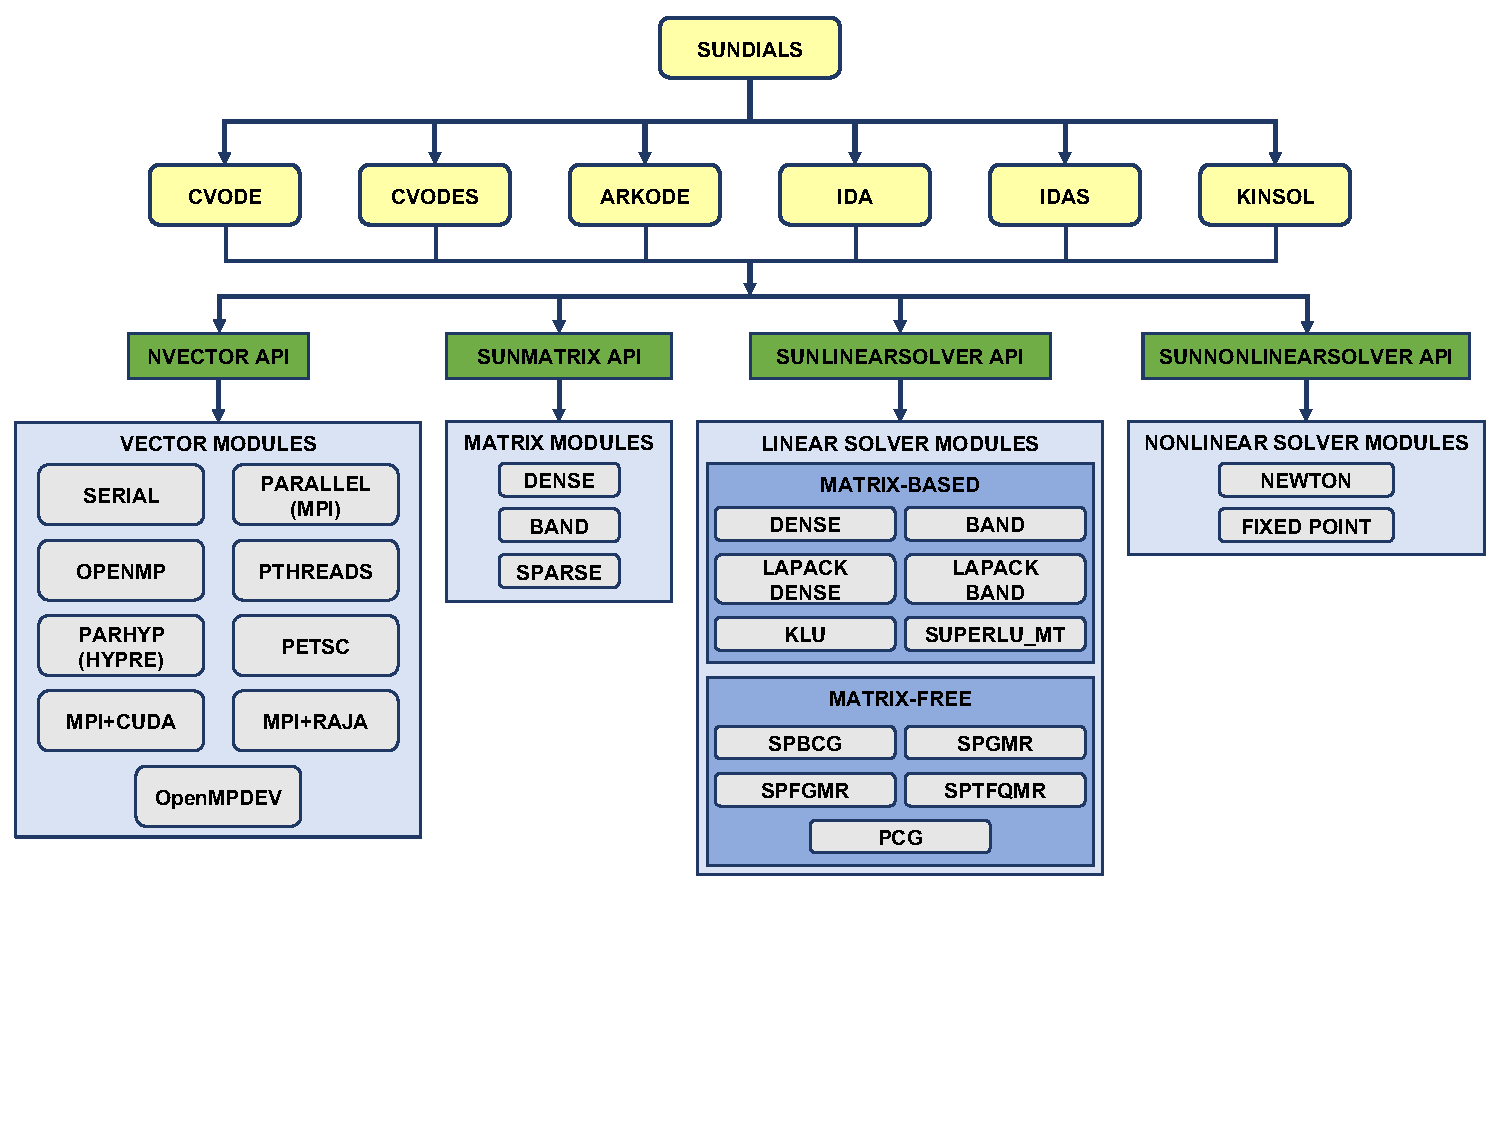
\includegraphics[width=6in]{projects/2.3.3-MathLibs/2.3.3.05-SUNDIALS/sunorg1.pdf}
	\caption{\label{fig:sunorg1}New structure of SUNDIALS showing options for the new SUNLINEARSOLVER and SUNMATRIX classes.}
\end{figure}

\paragraph{Next Steps}

During the remainder of FY18, this project team will:
\begin{enumerate}
\item Complete a release of SUNDIALS with the new fused vector routines implemented within each supplied vector and optionally used from the integrator packages.
\item Complete a release of SUNDIALS with all nonlinear solvers encapsulated and with implementations of the new nonlinear solver interfaces for both the Newton and fixed point solvers used in the integrator packages.
\end{enumerate}
